\subsection{A deterministic baseline for supplied preferences}
The receipt experiment asks models to recover information already in a structured input. A new offline control parses those supplied weights directly and checks membership in the declared four-profile taxonomy. It uses the same 720 field records across the nine conditions, without their private intent labels. The known identity channel eliminates report-calibration uncertainty. With $\alpha_q=.04$, field-frequency bounds resolve seven of nine comparisons, with zero incorrect resolutions and mean width 0.02285. There are no calibration observations or new API calls. A direct Hoeffding interval for the bounded variable $d_Z$, using the same $.04$ error budget, also resolves seven; its mean width is 0.02727. The methods are reported separately, not intersected.

This baseline changes the engineering interpretation of the receipt result. Given these structured inputs, routing the supplied attribute through an LLM and estimating its error channel is unnecessary. Preserving the field is simpler and produces more decisive intervals in this selected benchmark. It still does not validate the supplied profile against a real customer. These reanalyses use the previously selected field draws and remain exploratory.

\subsection{Structural ambiguity versus finite precision}
A separate controlled simulation isolates limitations conflated by the primary model experiment. Let
\begin{equation}
 A_\eta=(1-\eta)\mathbf1\mathbf1^T/4+\eta I_4,
 \quad d=(.06,.02,-.04,-.02)^T.
\end{equation}
The channel eigenvalues are $1,\eta,\eta,\eta$. At $\eta=0$, every population has the same action law and the compatible contrast interval is $[-.04,.06]$. For every $\eta>0$, $A_\eta$ is invertible and the exact-observation interval has zero width. Identification alone therefore does not describe the difficulty of the finite-sample inverse problem.

For known $A_\eta$ and $\eta>0$, write $\bar d=\mathbf1^Td/4$. The weights $v=\bar d\mathbf1+(d-\bar d\mathbf1)/\eta$ satisfy $A_\eta^Tv=d$, with range $\operatorname{range}(d)/\eta$. The certificate in Section~5.2 gives error at most
\begin{equation}
 \frac{\operatorname{range}(d)}{\eta}
 \sqrt{\frac{\log(2/\alpha)}{2n}}.
\end{equation}
Thus $n\geq\operatorname{range}(d)^2\log(2/\alpha)/(2\eta^2\epsilon^2)$ suffices for radius $\epsilon$ with these fixed weights. This is a sufficient Hoeffding bound, not an optimal sample-complexity or impossibility claim. Channel estimation adds another uncertainty source.

The sweep uses $\eta\in\{0,.01,.03,.1,.3,1\}$, calibration counts per class $c\in\{40,160,640,2560\}$, field counts $2c$, and the three original population mixtures. Each of 72 cells has 200 independent complete repetitions, totaling 14,400 multinomial simulations and 43,200 interval calculations. The three methods use exact $A$ with uncertain field frequencies, uncertain $A$ with exact $q$, or uncertainty in both. The first two have 98\% marginal guarantees, and the joint procedure has 96\%; these are uncertainty-source ablations, not an equal-confidence ranking. Methods share samples within a repetition; repetitions and cells use independent streams. All outcomes are constructed, and no new model or human observations are generated.

For the positive mixture with $\eta=.01$, even $c=2560$ and 5,120 field observations leave every joint interval unresolved: the median width remains .10 although structural width is zero. At $\eta=.1$ and the same counts, field-only, calibration-only, and joint resolution rates are 98\%, 54\%, and 1\%, respectively. The joint median width is 0.07651. These examples expose calibration and weak-signal costs; they do not identify the unknown population channels of the earlier LLM experiment.

All cells and repetitions are released. Coverage and resolution denominators retain infeasible cases; width quantiles condition on feasibility. There are 84 infeasible intervals and four incorrect resolutions, all in the field-only ablation. Observed field-only coverage ranges from 96\% to 100\% across cells, with Monte Carlo errors and exact binomial intervals reported. All joint and calibration-only intervals contain the target in these runs. A 200/200 count has a two-sided 95\% binomial lower bound of approximately .982, so it is not evidence of perfect coverage. No simultaneous claim over cells is made.

\begin{figure*}[t]
\centering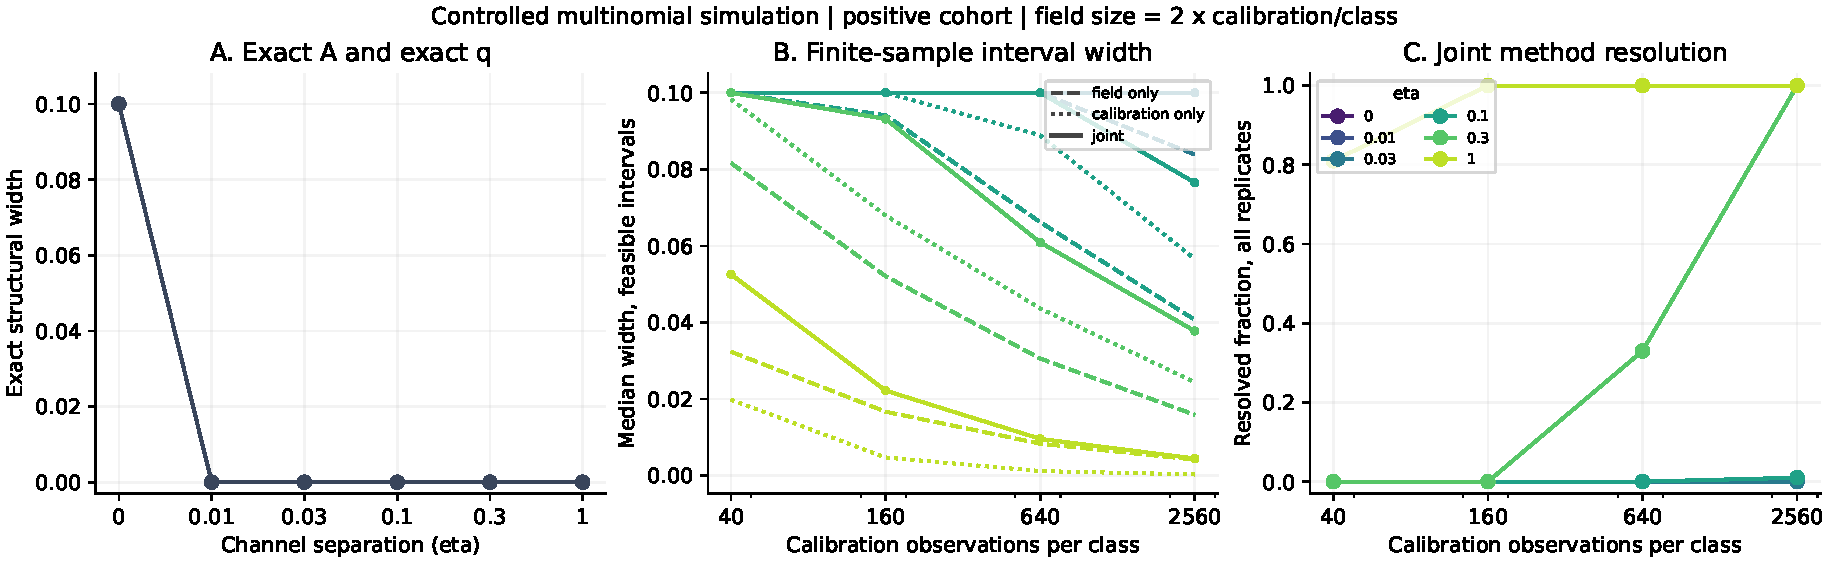
\includegraphics[width=.98\textwidth]{../results/precision-sweep-v3/precision-sweep.pdf}
\caption{Controlled separation of structural and statistical limitations. The figure displays the positive mixture; all three mixtures are in the released tables. Exact identification at every $\eta>0$ coexists with wide finite-sample intervals. Width summaries condition on feasibility; resolution denominators retain all repetitions. These are multinomial simulations, not additional LLM calls.}
\label{fig:precision}
\end{figure*}
